\documentclass[a4paper]{oblivoir}

\title{Chapter 12. Gaussian Process}
\author{\makebox[.9\textwidth]{Moon Il-chul}\\ \href{mailto:icmoon@kaist.ac.kr}{icmoon@kaist.ac.kr}
\and Na Yeong-yeon\\ \href{mailto:duddus15@kaist.ac.kr}{duddus15@kaist.ac.kr}
\and Kim Hyemi\\ \href{mailto:khm0308@kaist.ac.kr}{khm0308@kaist.ac.kr}}
\setcounter{chapter}{12}

\usepackage{indentfirst}
\usepackage{graphicx}
\graphicspath{ {Figure/} }
\usepackage{subcaption}
\usepackage{hyperref}
\usepackage{amsmath}
\usepackage{amssymb}
\usepackage{amsfonts}
\usepackage{dsfont}
\usepackage[]{algorithm2e}
\usepackage{chngcntr}
\counterwithin{figure}{chapter}
\setcounter{tocdepth}{2}
\setcounter{secnumdepth}{3}
\hypersetup{pdfborder={0 0 0}}
\renewcommand{\thefigure}{\thechapter-\arabic{figure}}
\renewcommand{\theequation}{\thechapter.\arabic{equation}}
\newlength\myindent
\setlength\myindent{5em}

\begin{document}

\maketitle

\tableofcontents
\newpage

%\chapter{}
%-----------------------------------------------------------------
\section{Simple Continuous Domain Analysis}
%-----------------------------------------------------------------

%-----------------------------------------------------------------
\subsection{Continuous Domain Data}
%-----------------------------------------------------------------

% 슬라이드 1
현실 세계의 많은 데이터들은 연속된 도메인을 가진다. 주가 지수, 시간, 공간, 시공간 등이 대표적인 예이다. 그러나 관측된 데이터는 불연속적인데, 이러한 경우는 관측된 데이터를 바탕으로 잠재 함수를 추정하여 분석할 수 있다.\\

\begin{figure}[ht] \centering 
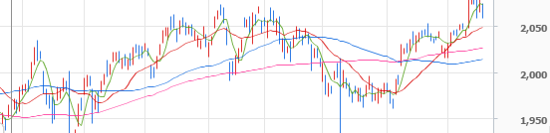
\includegraphics[scale=0.6]{fig12_1.png} 
\caption{연속된 시간에 따른 주가지수}
\label{fig:12-1}
\end{figure} 

\begin{figure}[ht] \centering
\centering
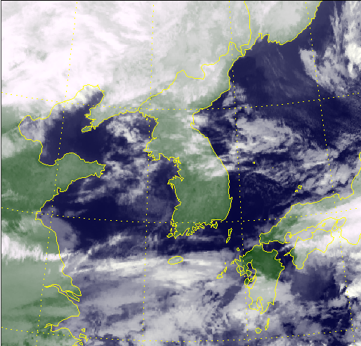
\includegraphics[scale=0.6]{fig12_2.png}\hspace{0.2cm}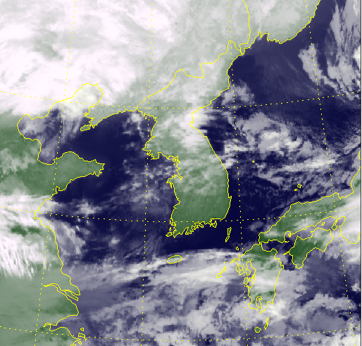
\includegraphics[scale=0.6]{fig12_3.png}
\caption{연속된 시공간에 따른 구름의 양}
\label{fig:12-2}
\end{figure}

%-----------------------------------------------------------------
\subsection{Underlying Function and Observations}
%-----------------------------------------------------------------

%슬라이드 6
잠재 함수를 추정하는데 사용되는 함수로 싱크함수가 있다. 싱크함수의 정의와 그래프는 다음과 같다.\\

\begin{equation}
sinc(x) = \frac{sin(\pi x)}{\pi x}
\label{eq:12-1}
\end{equation} 
\\

\begin{figure}[ht] \centering 
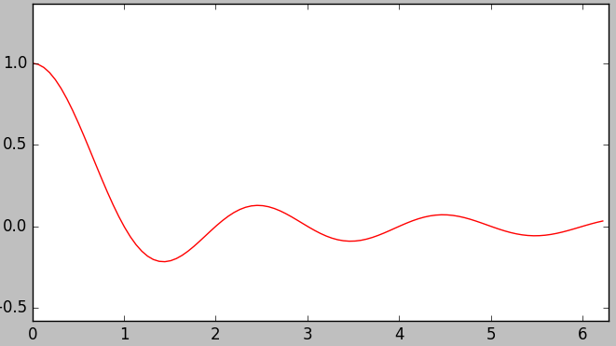
\includegraphics[scale=0.6]{fig12_4.png} 
\caption{싱크함수의 그래프}
\label{fig:12-3}
\end{figure} 

현실에서는 잠재 함수에 노이즈가 섞여 있다. 따라서 싱크함수에 가우시안 노이즈를 더한 형태를 잠재함수를 추정하는데 사용한다. 도메인의 한 점 $x_{i}$에 대한 가우시안 노이즈를 $e_{i}$ 라고 하면 데이터셋의 확률 분포는 다음과 같다.

\begin{equation}
e_{i} \sim N(o,\sigma_{i}^{2})
\label{eq:12-2}
\end{equation} 

이를 바탕으로 다음과 같은 두 가지 형태의 관찰데이터셋을 구성해 보겠다.\\

\begin{figure}[ht] \centering 
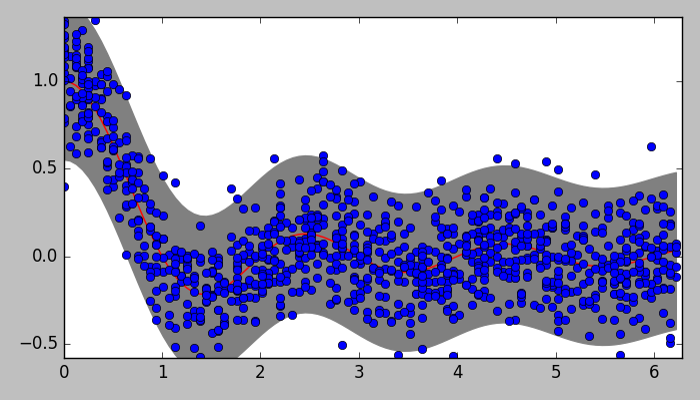
\includegraphics[scale=0.6]{fig12_5.png} 
\caption{싱크함수의 관찰데이터 1}
\label{fig:12-4}
\end{figure} 

\begin{figure}[ht] \centering 
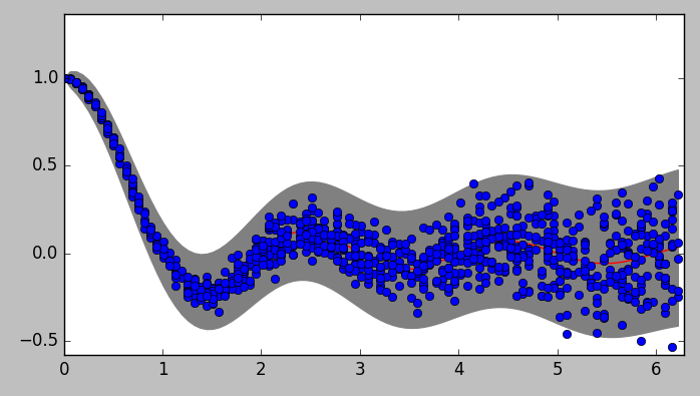
\includegraphics[scale=0.6]{fig12_6.png} 
\caption{싱크함수의 관찰데이터 2}
\label{fig:12-5}
\end{figure} 

두 데이터셋은 모두 싱크함수를 이용했음에도 불구하고 형태가 다르다. 그림 4의  데이터셋은 모든 $x_{i}$에 대해서  $\sigma_{i} = \sigma$로 일정한 분산 값을 가지는 반면 그림 5의 데이터셋은 $x_{i}$ 가 증가함에 따라 $\sigma_{i}$도 증가한다. 
이로부터 데이터 포인트에 따라 평균과 분산이 단순한 상수가 아니라 함수의 형태로 표현될 수 있음을 알 수 있다. 따라서 관측데이터를 통해 실제 잠재 함수를 추정하기 위해서는 에러항을 모델링해야 한다.

%-----------------------------------------------------------------
\subsection{Simple Analyses without Domain Correlation}
%-----------------------------------------------------------------

1.2 에서는 1000개의 관찰 데이터 포인트를 가지는 데이터셋이었다. 이번 단원에서는 50개의 관찰 데이터 포인트를 가지는 데이터셋을 그림 6과 같이 구성하였다.
\begin{figure}[ht] \centering 
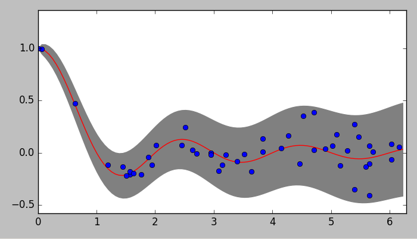
\includegraphics[scale=1]{fig12_7.png} 
\caption{싱크함수의 관찰데이터 3}
\label{fig:12-6}
\end{figure}

이제 그림 5와 그림 6의 데이터를 바탕으로 잠재함수를 추정해보도록 하겠다.\\
연속 도메인 중 하나의 포인트 $x_i$에 대한 관측값이 $t_{i1}$,$t_{i2}$,$\cdots$,$t_{ik}$ 라고 할 때 실제값 $y_{i}$는 다음과 같이 추정할 수 있다.\\

\begin{equation}
y_{i} = \frac{1}{N}\sum_{j=1}^{k}t_{ij}\
\label{eq:12-3} 
\end{equation} 

\begin{equation}
N=|\left\{t_{i1},t_{i2},\cdots,t_{ik}\right\}|\
\label{eq:12-4}
\end{equation} 

이처럼 하나의 도메인 포인트에서의 관찰값들의 평균을 내는 방식으로 실제값을 추정할 수 있고, 이렇게 추정한 잠재함수의 그래프는 다음과 같다.\\

\begin{figure}[ht] \centering 
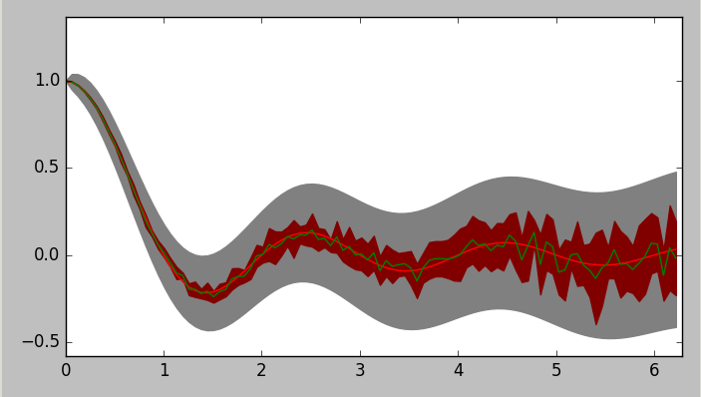
\includegraphics[scale=0.58]{fig12_8.png} 
\caption{관찰데이터2 (그림 5)의 추정된 잠재함수}
\label{fig:12-7}
\end{figure}

\begin{figure}[ht] \centering 
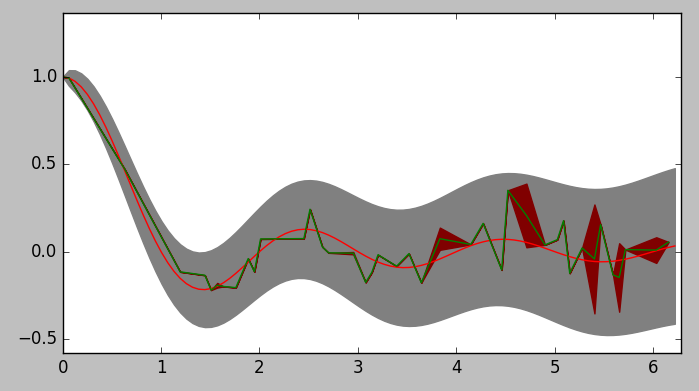
\includegraphics[scale=0.58]{fig12_9.png} 
\caption{관찰데이터3 (그림 6)의 추정된 잠재함수}
\label{fig:12-8}
\end{figure}

그림 7의 추정된 함수는 실제 함수가 비슷해 보인다. 이는 이용한 추정 방식이 적합함을 의미한다. 그러나 이를 추정하는데 사용된 그림 5와 같은 관측데이터는 현실에서 접하기 어렵다. 왜냐하면 현실 세계에서는 일반적으로 하나의 도메인 포인트에 대해 한 개 이하의 관찰값만 존재하기 때문이다. 예를 들어 한 개의 센서가 시간별 관찰값을 얻는다고 가정할 때, 특정 시간에 센서의 여러 관찰값을 얻는 것은 불가능하다.\\
그렇다면 그림 8을 살펴보자. 이 데이터셋에서는 하나의 도메인 포인트에 하나의 관찰값 밖에 없기 때문에 실제값 $y_{i}$는 다음과 같은 값을 가진다.

\begin{equation}
y_{i} = t_{i}\
\label{eq:12-5}
\end{equation} 
 
그러나 이는 관찰값이 실제값과 동일할 것이라는 단순한 추정이며 관측값들을 직선으로 이어놓은 것에 불과하다.이 추정 방법의 문제점은 도메인 정보를 전혀 사용하지 않은 것이다. 즉, 과거의 관찰값이 현재의 관찰값에 영향을 미칠 수 있음에도 불구하고 사용하지 않았다.\\

%-----------------------------------------------------------------
\subsection{Simple analyses with Domain Correlation }
%-----------------------------------------------------------------

이제부터는 추정에 현실세계에서 있을법한 데이터인 그림 6의 데이터셋만을 활용하겠다. 여기에서는, 과거의 관찰값이 현재의 관찰값에 영향을 미칠 수 있다는 사실을 감안하여, 도메인 사이의 관계를 고려한 이동 평균(Moving Average)을 활용한다.\\
이동 평균이란, 시계열의 각 지점에 대하여 그것을 중심으로 하는 전후 일정 지점의 평균값을 구하여 경향성을 도출하는 방법이다. 연속 도메인 위의 한 점 $x$에 대해 $x$의 앞 뒤로 도메인을 어느정도 고려할지는 time window $[w_{low}, w_{high}]$를 설정하여 정한다. 연속 도메인 위의 한 점 $x$에 대해 time window $[w_{low}, w_{high}]$와 도메인의 집합 $D$에 대한 이동 평균은 다음과 같이 정의된다.\\

\begin{equation}
MA(x) = \frac{1}{N}\sum_{x_{i}\in W,D}t_{i}\
\label{eq:12-6}
\end{equation} 

\begin{equation}
W= [x - w_{low}, x+w_{high}], \quad  N= |\left\{x_{i}|x_{i} \in W,D \right\}| \
\label{eq:10-2-3}
\end{equation} 

그리고 time window가 각각$[-\frac{2 \pi}{100} \times10,\frac{2 \pi}{100} \times10]$, $[-\frac{2 \pi}{100} \times10,\frac{2 \pi}{100} \times10]$, $[-\frac{2 \pi}{100} \times20,\frac{2 \pi}{100} \times20]$와 같은 값을 가질 때 추정한 잠재 함수는 다음과 같다.\\

\begin{figure}[ht] \centering 
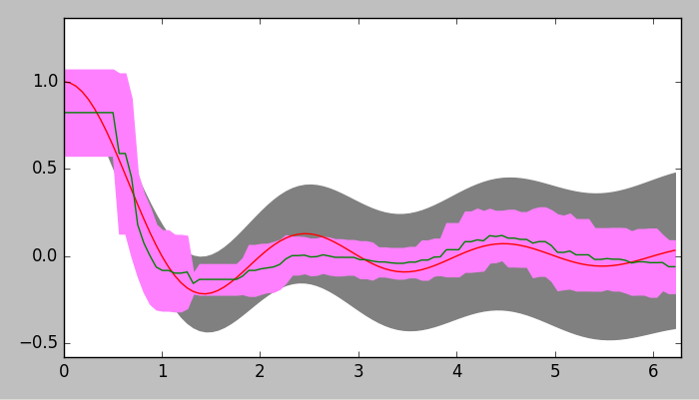
\includegraphics[scale=0.45]{fig12_10.png} 
\caption{time window $W = \left[-\frac{2 \pi}{100} \times10,\frac{2 \pi}{100} \times10\right]$ 일 때 추정된 잠재함수}
\label{fig:12-9}
\end{figure}

\begin{figure}[ht] \centering 
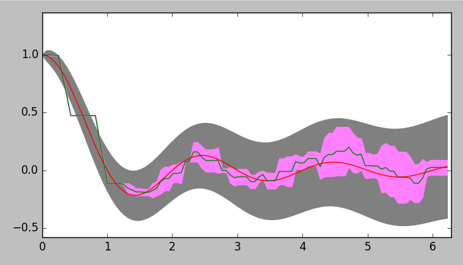
\includegraphics[scale=0.65]{fig12_11.png} 
\caption{time window $W = \left[-\frac{2 \pi}{100} \times3,\frac{2 \pi}{100} \times3\right]$ 일 때 추정된 잠재함수}
\label{fig:12-10}
\end{figure}

\begin{figure}[ht] \centering 
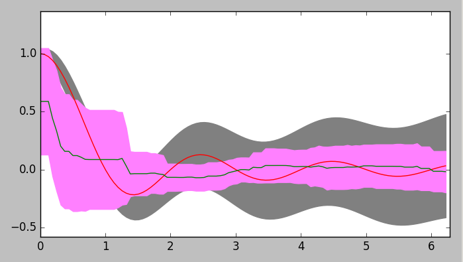
\includegraphics[scale=0.65]{fig12_12.png} 
\caption{time window $W = \left[-\frac{2 \pi}{100} \times20,\frac{2 \pi}{100} \times20\right]$ 일 때 추정된 잠재함수}
\label{fig:12-11}
\end{figure}

그림 9, 10, 11에서 살펴볼 수 있 듯, time window $W$의 크기에 따라 추정된 잠재 함수가 다르며 여기서 적절한 time window $W$가 무엇인지 판볋하기 어렵다. 또한 이동평균식에서의 가중치는 모두 1로 $W$ 안에 있는 관측값이라면 하루 전의 관측값이든 10년 전의 관측값이든 같은 가중치로 평균을 구한다는 점 또한 이동 평균 방식이 가지는 한계점이다.

%-----------------------------------------------------------------
\subsection{Simple Analyses with Differentiated Domain Correlation}
%-----------------------------------------------------------------

앞의 문제를 해결하기 위해 이동 평균을 낼 때의 $t_{i}$의 가중치를 1이 아닌 $x$와 $x_i$의 거리에 따라 다르게 조절하였다.\\
먼저 그림 12와 같이 가중치가 선형적인 경우, 이를 바탕으로 추정한 잠재함수는 실제 값을 이전보다 더 잘 추정한다. 그러나 선형가중치의 경우에는 미분값을 구할 수 없는 지점이 존재하며 구현하는데 구간에 따라 그래프를 설정해주어야 하는 한계를 지닌다.

\begin{figure}[ht] \centering
\centering
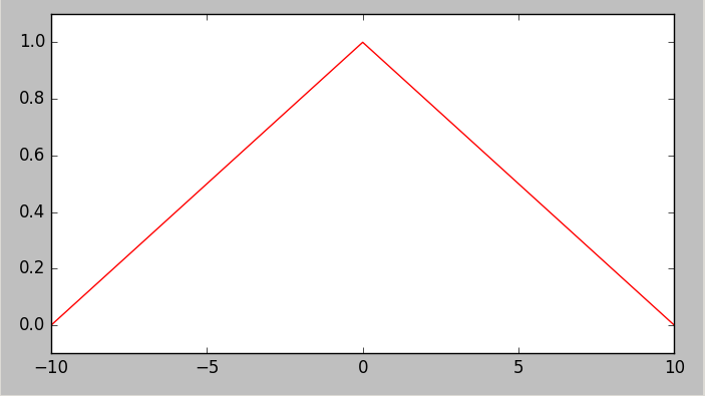
\includegraphics[scale=0.30]{fig12_26.png}\hspace{0.1cm}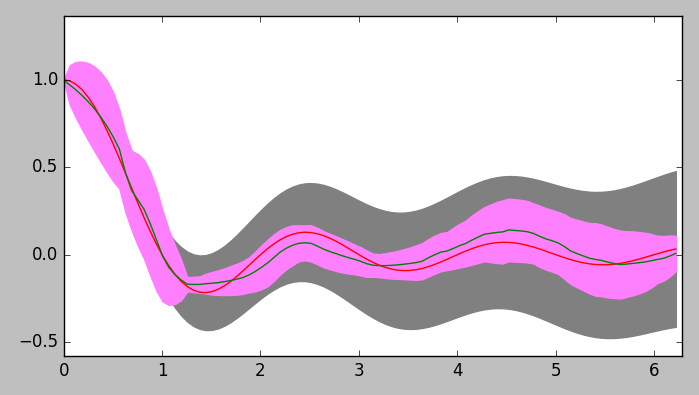
\includegraphics[scale=0.30]{fig12_27.png}
\caption{선형가중치 및 선형가중치로 추정한 잠재함수}
\label{fig:12-12}
\end{figure}

이러한 문제점을 해결하기 위해 그림 12와 같이 squared exponential 함수를 사용하여 잠재함수를 추정한다. 

squared exponential 함수는 연속 도메인 위의 한 $x$점 $x_{i}$와 에 대해 커널 함수로 $k(x, x_{i}) = exp\left(- \frac{{\left|x-x_{i} \right|}^{2}}{L^{2}} \right)$을 가진다. 이를 활용하여 도메인의 집합 $D$에 대한 이동 평균을 다음과 같이 정의할 수 있다.\\

\begin{equation}
MA(x) = \frac{1}{\sum_{x_{i} \in D}k(x,x_{i})}\sum_{x_{i} \in D}k(x,x_{i})t_{i}\
\label{eq:12-7}
\end{equation} 
 
여기서 time window가 식에 나타나지 않는 이유는 커널 함수에 의해 $x$와 $x_{i}$ 사이의 거리가 $L$보다 커질 경우 값이 0으로 정의된다. 즉, 커널함수의 정의 속에 time window가 숨어있다고 볼 수 있다.\\

\begin{figure}[ht] \centering
\centering
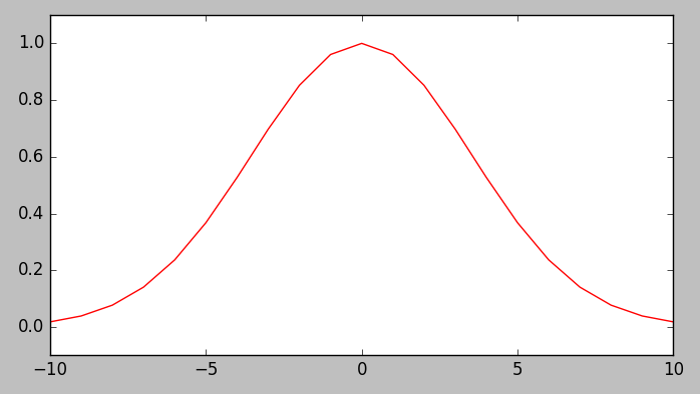
\includegraphics[scale=0.30]{fig12_25.png}\hspace{0.1cm}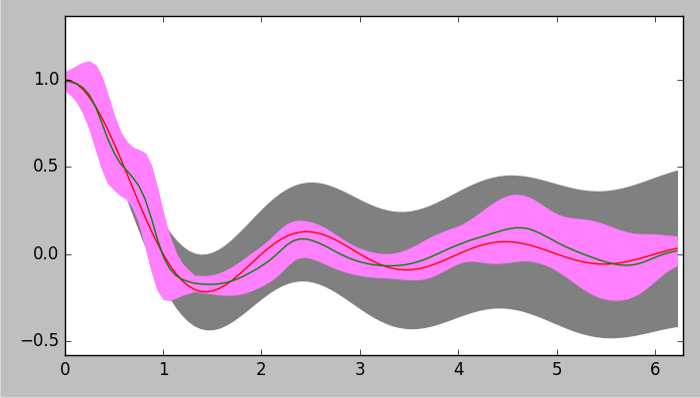
\includegraphics[scale=0.30]{fig12_13.png}
\caption{선형가중치 및 선형가중치로 추정한 잠재함수}
\label{fig:12-13}
\end{figure}

\section{Derivation of Gaussian Process Regression}
%-----------------------------------------------------------------

%-----------------------------------------------------------------
\subsection{Multivariate normal distribution}
%-----------------------------------------------------------------

지금까지 관찰된 데이터셋을 바탕으로 잠재함수를 추정하는 몇가지 방법을 알아보았다. 가우시안 프로세스 리그레션 역시 이와 같은 맥락이다. 먼저, 가우시안 프로세스란 연속 도메인 위의 $N$개의 포인트들의 집합 $X_{N} = [x_{1},x_{2}, \cdots , x_{N}]^{T}$에 대해 관찰된 포인트 집합을 $T_{N} = [t_{1},t_{2}, \cdots , t_{N}]^{T}$라 할 때, $T_{N}$이 다변수정규분포를 따르는 것을 의미한다. 여기서 가우시안 프로세스 리그레션은 주어진 $T_{N}$을 바탕으로 다음에 관찰될 값  $t_{n+1}$을 유추하는 것이 목표이다. 이 목표는 $T_{N}$을 바탕으로 $t_{N+1}$의 확률분포인 $P(t_{N+1}|T_{N})$을 찾음으로써 달성 될 수 있다.\\

따라서 가우시안 프로세스 리그레션에 대해 알아보기 전에, 그 바탕이 되는 다변수 정규분포에 대해 먼저 알아보겠다. $k$차원의 랜덤 벡터 $X =[X_{1}, X_{2}, \cdots , X_{k}]^{T}$ 가 다변수 정규분포를 따를 때 평균벡터, 공분산 행렬, 확률밀도 함수는 다음과 같이 표현된다.\\

\begin{equation}
X  \sim  N(\mu,\Sigma) \
\label{eq:12-8}
\end{equation} 

$X$가 위와 같은 분포일 때 $k$차원의 평균 벡터는 다음과 같다.

\begin{equation}
\mu = E[X] = \left[E[X_{1}], E[X_{2}], \cdots , E[X_{k}]\right]^{T}\
\label{eq:12-9}
\end{equation} 

$k\times k$ 차원의 공분산 행렬은 다음과 같이 나타난다.

\begin{equation}
\Sigma =: E \left[(X -\mu)(X=\mu)^{T} \right] = \left[Cov[X_{i},X_{j};1 \leq i,j \leq l.]  \right]\
\label{eq:12-10}
\end{equation} 

마지막으로 확률밀도함수(PDF)는 다음과 같다.

\begin{equation}
P(X) = \frac{1}{(2 \pi) ^{d/2}} \frac{1}{|\Sigma|^{1/2}}exp\left(-\frac{1}{2}(X -\mu)^{T} \Sigma^{-1}(X- \mu)\right)\
\label{eq:12-11}
\end{equation} 

추가적으로, 다변수 정규분포는 다음과 같은 성질을 따른다.\\

랜덤 벡터  $X = [X_{1} \quad X_{2}]^{T}$가 $X \sim N(\mu , \Sigma )$을 따르고,\\

$\mu =[\mu_1 \quad \mu_2]^{T}$, $\Sigma = \begin{bmatrix} \Sigma_{11} &\Sigma_{12}\\ \Sigma_{21} & \Sigma_{22} \end{bmatrix}$ 일 때,

\begin{equation}
P(X_{1}) = N(X_{1}|\mu_{1}, \quad \Sigma_{11})
\label{eq:12-12}
\end{equation} 

\begin{equation}
P(X_{1}|X_{2}) = N(X_{1}|\mu_{1} + \Sigma_{12}\Sigma_{22}^{-1}(X_{1}-\mu_{2}), \quad \Sigma_{11} - \Sigma_{12}\Sigma_{22}^{-1}\Sigma_{21})
\label{eq:12-13}
\end{equation} 

위 두 공식은 앞으로 다변수 정규분포를 다루는데 유용하게 쓰일 것이다.\\

%-----------------------------------------------------------------
\subsection{Linear Regression with Basis Function}
%-----------------------------------------------------------------

이전 단원에서 잠재함수 Y를 유추해보았다면, 이번 단원에서는 Y의 확률분포를 구해보겠다. 연속 도메인 위의 $N$개의 포인트들의 집합 $X_{N} = [x_{1},x_{2}, \cdots , x_{N}]^{T}$ 이 $M$차원으로 매핑되며 그 때의 $M$차원의 웨이트 벡터를 $W$, 매핑된 값을 $Y_{N} = [y_{1},y_{2}, \cdots , y_{N}]^{T}$라고 했을 때, $Y_{N}$는 다음과 같은 수식으로 나타낼 수 있다.\\

\begin{equation}
y(x_{i}) = W^{T}\phi (x_{i})
\label{eq:12-14}
\end{equation} 
\begin{equation}
W = [w_{1},w_{2}, \cdots , w_{M}]^{T}, \quad \phi(x_{i}) =[\phi_{1}(x_{i}), \phi_{2}(x_{i}), \cdots, \phi_{M}(x_{i})]^{T}
\label{eq:12-15}
\end{equation} 


모든 원소 $(x_{1},y_{1}),(x_{1},y_{1}), \cdots, (x_{N},y_{n})$에 대해 식 15를 행렬곱으로 표현하면 아래와 같이 표현된다.

\begin{eqnarray}
Y & = & \Phi W\nonumber\\
& = & \begin{bmatrix} \phi(x_{1})^{T} \\ \phi(x_{2})^{T} \\ \vdots \\ \phi(x_{N})^{T} \end{bmatrix} \begin{bmatrix} w_{1} \\ w_{2} \\ \vdots \\ w_{M}
\end{bmatrix}\nonumber\\
& = & \begin{bmatrix} \phi_{1}(x_{1}) & \phi_{2}(x_{1}) & \cdots & \phi_{M}(x_{1})  \\ \phi_{1}(x_{2}) & \phi_{2}(x_{2}) & \cdots & \phi_{M}(x_{2}) \\ \vdots & \vdots & \ddots & \vdots\\ \phi_{1}(x_{N}) & \phi_{2}(x_{1}) & \cdots & \phi_{M}(x_{1}) \end{bmatrix} \begin{bmatrix} w_{1} \\ w_{2} \\ \vdots \\ w_{M}
\end{bmatrix}
\end{eqnarray} 

전에는 $W$를 고정된 값으로 가정했지만, 이제는 이를 확률적으로 분포된 값으로 가정하겠다. $W$의 확률분포는 다음과 같이 정의한다. 

\begin{equation}
P(W) =N(W|0,\alpha^{-1}I)
\label{eq:12-16}
\end{equation} 

$W$와 $Y$는 식 15와 같이 표현되므로, $W$의 확률분포를 이용해서 $Y$의 확률분포를 구할 수 있다.

\begin{equation}
E[Y] = E[\Phi W] = \Phi E[W]
\label{eq:12-17}
\end{equation} 

\begin{equation}
cov[Y] = E[(Y -0)(Y -0)^{T}] =E[YY^{T}] = E[\Phi W W^{T} \Phi^{T}]= \Phi E[WW^{T}] \Phi  = \frac{1}{\alpha}\Phi \Phi^{T}
\label{eq:12-18}
\end{equation} 

공분산 행렬의 원소를 다음과 같은 커널함수로 정의하면 다음과 같이 나타난다.

\begin{equation}
K_{nm} = k(x_{n}, x_{m}) = \frac{1}{\alpha}\phi(x_{n}) \phi(x_{m} )
\label{eq:12-19}
\end{equation} 

따라서, $Y$의 확률 분포를 정리하면 다음과 같다.

\begin{equation}
P(Y) =N(W|0,K)
\label{eq:12-20}
\end{equation} 

%-----------------------------------------------------------------
\subsection{Modeling Noise With Gaussian Distribution}
%-----------------------------------------------------------------

2.2에서 $Y$의 확률분포에 대해 알아보았다. 그렇다면 $Y$는 $P(t_{N+1}|T_{N})$을 유추하는데 어떤 역할을 하는가? 연속 도메인의 하나의 포인트 $x_{n}$에 대해 실제로 관측된 값을 $t_{n}$, 가우시안 에러를 $e_{n}$이라고 하면 변수들끼리 다음과 같은 관계가 성립한다.

\begin{equation}
t_{n} = y_{n} +e_{n}
\label{eq:12-21}
\end{equation} 

정규분포의 성질에 따라 조건부 확률 분포는 다음과 같다.\\ 
\begin{equation}
P(t_{n} | y_{n}) =N(t_{n} | y_{n}, \quad \beta^{-1})
\label{eq:12-22}
\end{equation} 

이를 모든 원소들에 대한 행렬로 나타내면 아래와 같다.\\

\begin{equation}
P(T| Y) =N(T | Y, \quad \beta^{-1}I_{N})
\label{eq:12-23}
\end{equation} 

%-----------------------------------------------------------------
\subsection{Marginal Gaussian Distribution }
%-----------------------------------------------------------------
조건 분포 $P(T|Y)$를 바탕으로 $P(T)$를 구할 수 있다. 일반적으로는 $T$와 $Y$의 결합 분포를 $Y$에 대해 적분하여 구할 수 있다.\\
\begin{equation}
P(T) = \int P(T|Y)P(Y)dY =\int N(T|Y,\beta^{-1}I_{N})N(Y|0,K)dY
\label{eq:12-24}
\end{equation} 

하지만 우리는 2.1에서 나왔던 다변수 정규분표의 성질을 이용하여 구해보도록 하겠다. 먼저 $P(T|Y)P(Y) = P(T,Y) = P(Z)$라고 정의하고 자연로그를 씌워서 간단히 하면 다음과 같다.

\begin{eqnarray}
\ln P(Z) & = & \ln P(Y) + \ln P(T|Y)\nonumber\\
& = & -\frac{1}{2}(Y-0)^{T}K^{-1}(Y-0) -\frac{1}{2}(T-Y)^{T}\beta I_{N}(T-Y) +const \nonumber\\
& = & -\frac{1}{2}(Y)^{T}K^{-1}(Y) -\frac{1}{2}(T-Y)^{T}\beta I_{N}(T-Y) +const \nonumber\\
\label{eq:12-25}
\end{eqnarray} 

상수를 제외하고 간단히 하면 다음과 같이 나타난다.

\begin{eqnarray}
\textrm{given equation} & = & \ln P(Y) + \ln P(T|Y)\nonumber\\
& = & -\frac{1}{2}Y^{T}K^{-1}Y -\frac{\beta}{2}T^{T}T +\frac{\beta}{2}TY +\frac{\beta}{2}YT -\frac{\beta}{2}Y^{T}T \nonumber\\
& = & -\frac{1}{2} \begin{pmatrix} Y \\  T \end{pmatrix}^{T} \begin{pmatrix} K^{-1} + \beta I_{N} & -\beta I_{N} \\ -\beta I_{N} & \beta I_{N} \end{pmatrix}\begin{pmatrix} Y \\ T \end{pmatrix}\nonumber\\
& = & -\frac{1}{2}Z^{T}RZ \nonumber \\
\label{eq:12-26}
\end{eqnarray} 

그런데 이 형태는 2.1에서 보았던 다변수 정규분포의 확률밀도함수(PDF)에 자연로그를 씌운 형태와 같다. 따라서 $Z$ 는 평균 벡터가 0벡터, 공분산 행렬을 $R^{-1}$로 갖는 다변수 정규분포를 따른다.\\
공분산 행렬인 $R^{-1}$를 구할 때, 부분행렬로 이루어진 행렬의 역행렬을 구하는 아래의 공식을 이용할 수 있다.\\

\begin{equation}를
\begin{pmatrix} A & B \\ C & D \end{pmatrix}^{-1} = \begin{pmatrix} M & -MBD^{-1} \\ -D^{-1}CM & D^{-1} +D^{-1}CMBD^{-1} \end{pmatrix}
\label{eq:12-27}
\end{equation}

\begin{equation}
M =(A -BD^{-1}C)^{-1}
\label{eq:12-28}
\end{equation} 

이를 이용하여 $R^{-1}$을 계산하면 다음과 같다.

\begin{equation}
M =(K ^{-1} +\beta I_{N} - \beta I_{N}(\beta I_{N})^{-1}\beta I_{N})^{-1} = K
\label{eq:12-29}
\end{equation} 

\begin{eqnarray}
R^{-1} & = & \begin{pmatrix} K & K \beta I_{N}(\beta I_{N})^{-1} \\ (\beta I_{N})^{-1}\beta I_{N}K & (\beta I_{N})^{-1} +(\beta I_{N})^{-1} \beta I_{N} K \beta I_{N}(\beta I_{N})^{-1} \end{pmatrix} \nonumber\\
& = & \begin{pmatrix} K & K \\ K & (\beta I_{N})^{-1}+K \end{pmatrix}
\label{eq:12-30}
\end{eqnarray} 

따라서 $Z$의 확률분포는 다음과 같이 나타난다.\\

\begin{equation}
P(Z) = N\left(Z | \space 0, \begin{pmatrix} K & K \\ K & (\beta I_{N})^{-1}+K \end{pmatrix} \right)
\label{eq:12-31}
\end{equation} 

위 식을 마탕으로 2.1에서 보았던 다변수 정규분포의 성질 식 \ref{eq:12-12}을 이용하여 결합분포$P(Y, T)$를 바탕으로 단일분포$P(T)$를 쉽게 구할 수 있다.

\begin{equation}
P(T) = N\left(T | 0, (\beta I_{N})^{-1} + K \right)
\label{eq:12-32}
\end{equation} 

%-----------------------------------------------------------------
\subsection{Mean and Covariance of \texorpdfstring{$P(t_{N+1}|T_{N})$}{Lg}}
%-----------------------------------------------------------------

2.4에서 구한 것처럼 $P(T) = N\left(T | 0, (\beta I_{N})^{-1} + K \right)$임으로 $T_{N} = [t_{1},t_{2}, \cdots , t_{N}]^{T}$에 새로 관측할 포인트 $t_{N+1}$을 추가한 벡터 $T_{N+1}$의 확률분포는 다음과 같다.
\begin{eqnarray}
P(T_{N+1}) & = & P(T_{N}, t_{N+1})\nonumber\\
& = & N\left(T | 0, \begin{pmatrix} (\beta I_{N})^{-1}+K & k_{1(N+1)} \\ K_{(N+1)1} & K_{(N+1)(N+1)} + \beta \end{pmatrix} \right)
\label{eq:12-33}
\end{eqnarray} 

\begin{equation}
cov_{N+1} = \begin{bmatrix} cov_{N} & k \\ K^{T} & c \end{bmatrix}
\label{eq:12-34}
\end{equation} 

또한 2.1에서 언급했던 식 \ref{eq:12-13}을 이용하여 결합분포를 알 때, 조건 분포를 쉽게 구할 수 있다. 

\begin{equation}
P(t_{N+1}|T_{N}) = N\left(t_{N+1} | 0 + k^{T}cov_{N}^{-1}(T_{N}-0), c- k^{T}cov_{N}^{-1}k \right)
\label{eq:12-35}
\end{equation} 

따라서 $\mu_{t_{N+1}}$과 $\sigma_{t_{N+1}}$은 $\mu_{t_{N+1}|T_{N}} =k^{T}cov_{N}^{-1}T_{N}$, $\sigma_{t_{N+1}|T_{N}} = c- k^{T}cov_{N}^{-1}k $와 같이 나타난다.

\subsection{Hyperparameters of Gaussian Process Regression}
%-----------------------------------------------------------------
지금까지 가우시안 프로세스 리그레션이 어떻게 유도되는지 살펴 보았다. 이제는 각각 다른 하이퍼파라미터의 값을 가진 가우시안 프로세스가 어떻게 회귀되는지 살펴보겠다.\\

\begin{figure}[ht] \centering 
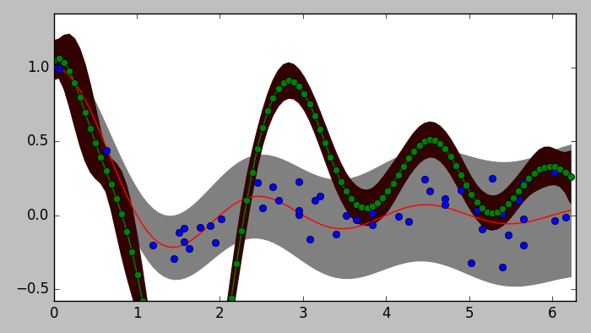
\includegraphics[scale=0.6]{fig12_14.png} 
\caption{$(\theta_{0},\theta_{0},\theta_{0},\theta_{0}, \beta ) = (0.5,10,0,0,0.01)$ 일 때의 가우시안 프로세스 리그레션}
\label{fig:12-14}
\end{figure}

\begin{figure}[ht] \centering 
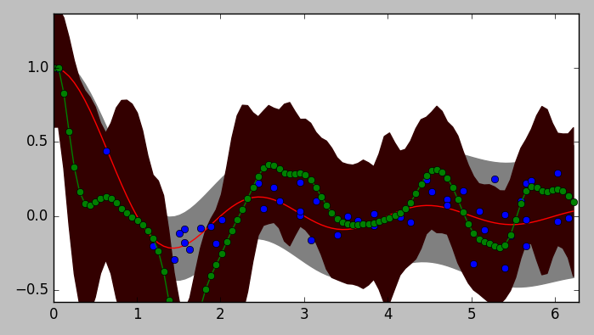
\includegraphics[scale=0.6]{fig12_15.png} 
\caption{$(\theta_{0},\theta_{0},\theta_{0},\theta_{0}, \beta ) = (0.5,50,0,0,0.01)$ 일 때의 가우시안 프로세스 리그레션}
\label{fig:12-15}
\end{figure}

위 그림을 통해 가우시안 프로세스 리그레션은 하이퍼 파라미터의 영향을 많이 받음을 알 수 있다. 즉, 하이퍼 파라미터를 학습시키지 않는다면 좋은 추정을 할 수 없다. 적합한 학습을 거친다면 다음과 같은 결과를 얻을 수 있다.\\

\begin{figure}[ht] \centering 
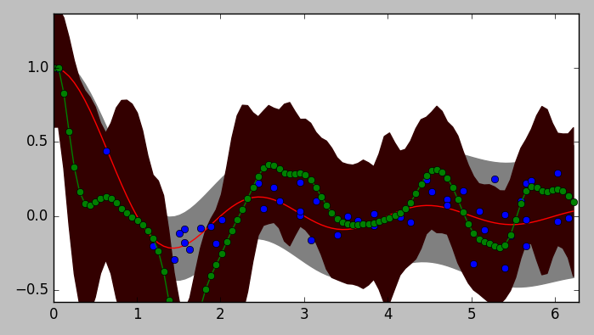
\includegraphics[scale=0.6]{fig12_15.png} 
\caption{$(\theta_{0},\theta_{0},\theta_{0},\theta_{0}, \beta ) = (1.377, 1.22, 1.354, 1.858, 9.980)$ 일 때의 가우시안 프로세스 리그레션}
\label{fig:12-16}
\end{figure}

%-----------------------------------------------------------------
\subsection{Probabilistic Programming for Hyperparameter Learning of GP}
%-----------------------------------------------------------------

다음과 같은 커널함수를 사용하여 커널 하이퍼파라미터를 텐서플로우라는 프레임워크를 이용하여 학습시켜 보겠다.
\begin{equation}
K_{nm}= k(x_{n}, x_{m}) =\theta_{0}exp \left( -\frac{\theta_{1}}{2} \parallel x_{n} - x_{m} \parallel^{2} \right) +\theta_{2} + \theta_{3}x_{n}^{T}x_{m}
\label{eq:12-36}
\end{equation} 

이러한 커널함수를 'KernelFunctionWithTensorFlow'로 정의하였다.

\begin{figure}[ht] \centering 
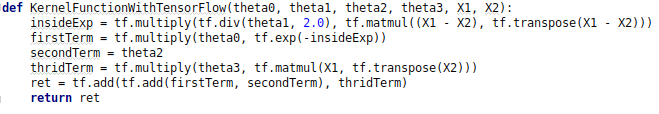
\includegraphics[scale=0.6]{fig12_18.png} 
\caption{커널함수를 KernelFunctionWithTensorFlow로 정의}
\label{fig:12-17}
\end{figure}

그림 18의 코드는 Covariance Matrix를 구성하는 과정을 포함하고 있으며, 그림 19의 코드는 관측된 데이터와 앞에서 구한 Covariance Matrix를 기반으로 다음 데이터 값을 예측하는 과정을 담고 있다.

\begin{figure}[ht] \centering 
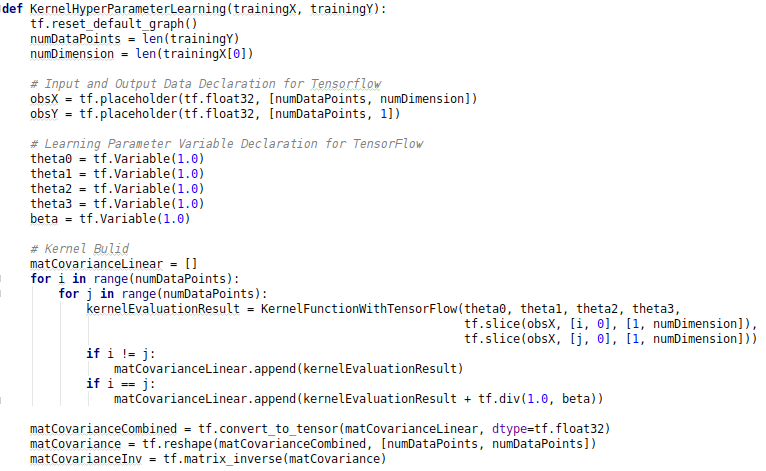
\includegraphics[scale=0.6]{fig12_17.png} 
\caption{하이퍼파라미터 학습 구현1}
\label{fig:12-18}
\end{figure}

\begin{figure}[ht] \centering 
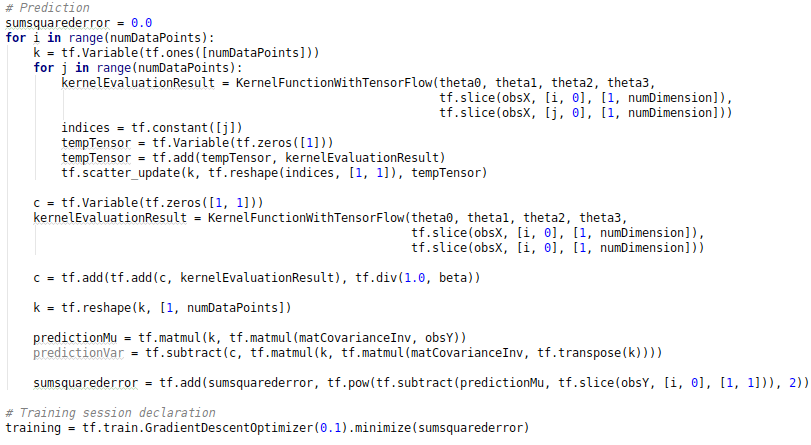
\includegraphics[scale=0.6]{fig12_19.png} 
\caption{하이퍼파라미터 학습 구현2}
\label{fig:12-19}
\end{figure}

%-----------------------------------------------------------------
\subsection{Bayesian Optimization with Gaussian Process}
%-----------------------------------------------------------------

지금까지 가우시안 프로세스 리그레션에 대해 알아보았다. 이제부터는 가우시안 프로세스를 적용할 수 있는 베이지안 최적화에 대해 알아보겠다. 베이지안 최적화는 우리가 순차적이고 입력값을 정할 수 있는 실험을 진행한다고 가정할 때, 결과값을 최대 혹은 최소로 만드는 입력값(input)을 찾는 것을 목표로 한다. 베이지안 최적화는 우리가 결과값을 결정하는 잠재함수를 모른다는 점, 결과값과 입력값이 연속적이다는 점, 결과값이 확률적(stochastic)으로 발생한다는 점이 특징이다. 베이지안 최적화의 목적을 수식으로 나타내면 아래와 같다.

\begin{equation}
x^{*} = argmax_{x \in X}f(x)
\label{eq:12-37}
\end{equation}

이러한 문제를 풀기 위한 기존에 알려진 방법에는 ‘Grid Search’가 있다. 이 방법은 도메인을 적당한 격자로 나누어 각각의 실험값을 찾아냄으로써 가장 큰 결과값을 찾아내는 방법이다. 다른 방법으로는 ‘Binary Search’가 있다. 이 방법은 하나의 실험값에 대해 양 옆의 실험값을 알아내어 결과값이 더 큰 방향으로 동일 과정을 진행하는 방법이다. 그러나 이 과정들은 잠재함수를 학습하여 최적값을 찾아내는 방식이 아니다.

베이지안 최적화는 잠재함수에 대해 학습하는 과정과 다음 샘플링 입력값을 선택하는 과정이 번갈아가며 일어나는 과정이다. 베이시안 최적화는 아래 4가지 연속되는 그림과 같이 이루어진다. 과정1-3에서는 분산을 줄여주게끔 샘플링하는 exploitation 과정을, 과정4에서는 평균이 커지는 지점을 반복하여 샘플링하는 exploration 과정을 수행하며 과정인 진행될수록 잠재함수가 실제함수와 유사하게 학습되는 것을 확인할 수 있다.\\

\begin{figure}[ht]
   \begin{subfigure}[b]{0.5\textwidth}
     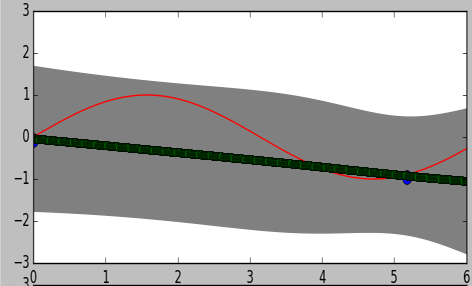
\includegraphics[width=\textwidth]{fig12_21.png}
     \caption{과정1}
   \end{subfigure}\hspace{0.1cm}
   \begin{subfigure}[b]{0.5\textwidth}
     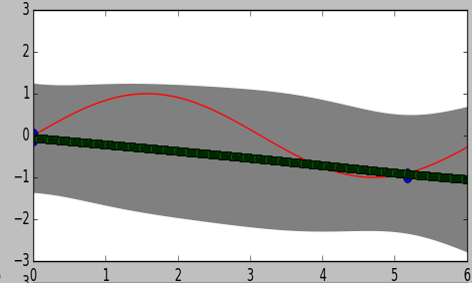
\includegraphics[width=\textwidth]{fig12_22.png}
     \caption{과정2}
   \end{subfigure}\\
   \begin{subfigure}[b]{0.5\textwidth}
     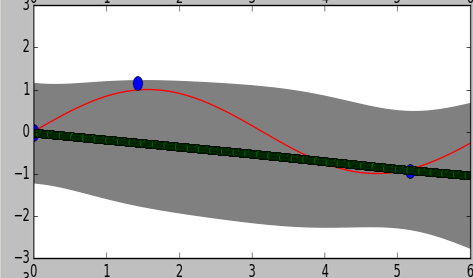
\includegraphics[width=\textwidth]{fig12_23.png}
     \caption{과정3}
   \end{subfigure}\hspace{0.1cm}
   \begin{subfigure}[b]{0.5\textwidth}
     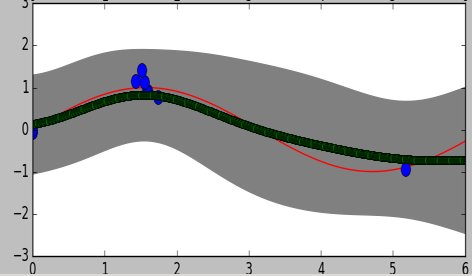
\includegraphics[width=\textwidth]{fig12_24.png}
     \caption{과정4}
   \end{subfigure}
   \caption{베이시안 최적화 과정}
   \label{fig:12-20}
\end{figure}

%-----------------------------------------------------------------
\subsection{Acquisition Function: Maximum Probability of Improvement}
%-----------------------------------------------------------------

이전 단원에서 exploitation과 exploration 사이에서 적절한 샘플링 방식을 선택하여 베이시안 최적화를 진행한다고 하였다. 여기서 적절한 샘플링 방식을 결정해주는 함수가 ‘Acquisition Function’이다. 가우시안 프로세스는 어느 포인트에서라도 예측된 평균과 표준편차값을 알려준다. 여기서 예측된 평균은 우리가 최적화된 값을 찾을 수 있다는 의미이고, 예측된 표준편차값은 예측의 리스크를 의미한다. 'Acquistion Function'은 이 두 요소를 고려하여 다음 샘플링 포인트를 찾아준다.\\

이러한 Aquisition Function에는 여러가지가 있는데 그 중에서 ‘Maximum Probability of Improvement’에 대해 알아보겠다. ‘Maximum Probability of Improvement’는 기존의 데이터 $D$가 가지고 있는 함수 $f(x)$의 최대값을 $y_{max}$, 새로운 샘플링 포인트 $x$를 잡았을 때의 합수값 $y=f(x)$라고 할 때,  $y$가 $y_{max}$보다  margin $m$만큼 혹은 더 크게 할 확률 중, 가장 높은 확률을 가지게 하는 $x$를 구하는 방법이다. 유도는 다음과 같다.

\begin{equation}
y \sim N(\mu, \sigma^{2}),\space CDF function \space\Phi 
\label{eq:12-38}
\end{equation}

\begin{align*}
MPI(x|D)&=argmax_{x}P(y \geq(1+m)y_{max}|x,D) \\
&=argmax_{x}P(\frac{y-\mu}{\sigma} \geq\frac{(1+m)y_{max}-\mu}{\sigma}) \\
&=argmax_{x}{1-\Phi(\frac{(1+m)y_{max}-\mu}{\sigma})} \\
&=argmax_{x}\Phi(\frac{\mu-(1+m)y_{max}}{\sigma}) \\
\label{eq:12-39}
\end{align*}

이 과정과 'Grid search'와의 차이점에 의문이 들 수 있다. 'Grid search'는 실제 실험을 진행하여 포인트들의 함수값을 실제로 계산하는 것이라면 ‘Maximum Probability of Improvement’는 실험을 수행하는 것이 아닌, 포인트들에 대한 누적분포값 $\Phi(\frac{\mu-(1+m)y_{max}}{\sigma})$만을 구하고 가장 높은 값을 가진 x를 다음 샘플링 포인트로 결정하는 과정이다.\\

%-----------------------------------------------------------------
\subsection{Acquisition Function: Maximum Expected Improvement}
%-----------------------------------------------------------------

다음으로 'Maximum Expected Improvement'에 대해 알아 보겠다. 이는 앞서 다뤘던 'Maximum Probability of Improvement'의 문제점을 보안한 것이다. 'Maximum Probability of Improvement'에서는 margin의 역할을 하는 하이퍼 파라미터 $m$ 역시 최적화 해주어야 한다. 따라서 'Maximum Expected Improvement'에서는 마진 $m$을 0에서 무한대까지 순차적으로 변화시킴으로써 m에 대한 평균값이 가장 큰 $x$를 구한다.

여기서는 다음과 같은 가정이 필요하다.
\begin{equation}
y =f(x), \quad y_{max} = \underset{m = 1,\cdots,n}{max}f(x_{n})\nonumber\\
\label{eq:12-40}
\end{equation}

\begin{equation}
u =\frac{y_{max}-\mu}{\sigma}, \quad v =\frac{u-\mu}{\sigma}\nonumber\\
\label{eq:12-41}
\end{equation}

\begin{equation}
\mu = f(x|D), \quad \sigma = K(x|D)\nonumber\\
\label{eq:12-42}
\end{equation}

\begin{equation}
m = max(0, y-y_{max}) = max(0,(v-u)\sigma)\nonumber\\
\label{eq:12-43}
\end{equation}

이 때, 아래와 같은 조건을 만족하는 $x$를 구한다.

\begin{equation}
MEI(x|D) = argmax_{x}\int_{0}^{\infty}P(y_{max}+ m)m dm
\label{eq:12-44}
\end{equation} 
이 식을 정리하면 아래와 같다.
\begin{equation}
\allowdisplaybreaks
\begin{aligned}
\int_{0}^{\infty}P(y \geq y_{max}+ m)m dm & = \int_{0}^{\infty}P(\frac{y-\mu}{\sigma} \geq \frac{y_{max} -\mu + m}{\sigma})m dm \nonumber\\
& = \int_{0}^{\infty}P(v \geq u + \frac{m}{\sigma})m dm \nonumber\\
& = \int_{0}^{\infty} \int_{u+\frac{m}{\sigma}}^{\infty}\phi(\tilde{v}) d\tilde{v} m dm \nonumber\\
& = \int_{0}^{\infty} \int_{0}^{\infty} \chi_{[u+\frac{m}{\sigma},\infty)}(\tilde{v})\phi(\tilde{v})d\tilde{v} m dm\nonumber\\
& = \int_{0}^{\infty} \int_{0}^{\infty} m\chi_{[u+\frac{m}{\sigma},\infty)}(\tilde{v})\phi(\tilde{v})d\tilde{v} dm\nonumber\\
& = \int_{0}^{\infty} \int_{0}^{\infty} m\chi_{[u+\frac{m}{\sigma},\infty)}(\tilde{v})\phi(\tilde{v})dm d\tilde{v}\nonumber\\
& = \int_{0}^{\infty} \bigg\{\int_{0}^{\infty} m\chi_{[u+\frac{m}{\sigma},\infty)}(\tilde{v})dm\bigg\}\phi(\tilde{v})dm d\tilde{v}\nonumber\\
& = \int_{0}^{\infty} \bigg\{\int_{0}^{\infty} m\chi_{\{0 \leq m \leq \sigma(\tilde{v}-u)\}}(\tilde{v}) dm \bigg\} \phi(\tilde{v})d\tilde{v}\nonumber\\
& = \int_{0}^{\infty} \bigg\{\int_{0}^{\infty} m\chi_{\{0 \leq m \leq \sigma(\tilde{v}-u)\} \cap \{0 \leq \sigma(\tilde{v}-u)\}}(\tilde{v}) dm \bigg\} \phi(\tilde{v})d\tilde{v}\nonumber\\
& = \int_{0}^{\infty} \bigg\{\int_{0}^{\infty} m\chi_{\{0 \leq m \leq \sigma(\tilde{v}-u)\}}(\tilde{v}) \chi_{\{\cap \{0 \leq \sigma(\tilde{v}-u)\}}(\tilde{v}) dm \bigg\} \phi(\tilde{v})d\tilde{v}\nonumber\\
& = \int_{0}^{\infty} \bigg\{\int_{0}^{\infty} m\chi_{\{0 \leq m \leq \sigma(\tilde{v}-u)\}}(\tilde{v}) dm \bigg\} \chi_{\{0 \leq \sigma(\tilde{v}-u)\}}(\tilde{v}) \phi(\tilde{v})d\tilde{v}\nonumber\\
& = \int_{u}^{\infty} \bigg\{\int_{0}^{\sigma(\tilde{v}-u)} m dm \bigg\} \phi(\tilde{v})d\tilde{v}\nonumber\\
& = \int_{u}^{\infty} \frac{1}{2} \sigma^{2} (\tilde{v}-u)^{2} \phi(\tilde{v})d\tilde{v}\nonumber\\
& = \frac{1}{2} \sigma^{2} \bigg[ \int_{u}^{\infty} \tilde{v}^{2} \phi(\tilde{v})d\tilde{v} - 2u \int_{u}^{\infty} \tilde{v} \phi(\tilde{v})d\tilde{v} + u^{2} \int_{u}^{\infty}\phi(\tilde{v})d\tilde{v} \bigg]\nonumber\\
& = \frac{1}{2} \sigma^{2} \bigg[ -u \phi(u) + (1+u^{2}) \Phi(-u) \bigg]
\label{eq:12-45}
\end{aligned}
\end{equation} 

아래의 그림은 베이지안 최적화 과정에서 Maximum Expected Improvement로 샘플링을 진행했을 때 iteration에 따라 샘플링되어 학습된 함수와 Probability Improvment 함수와 Expected Improvment 함수를 나타낸 결과다.

\begin{figure}[ht]
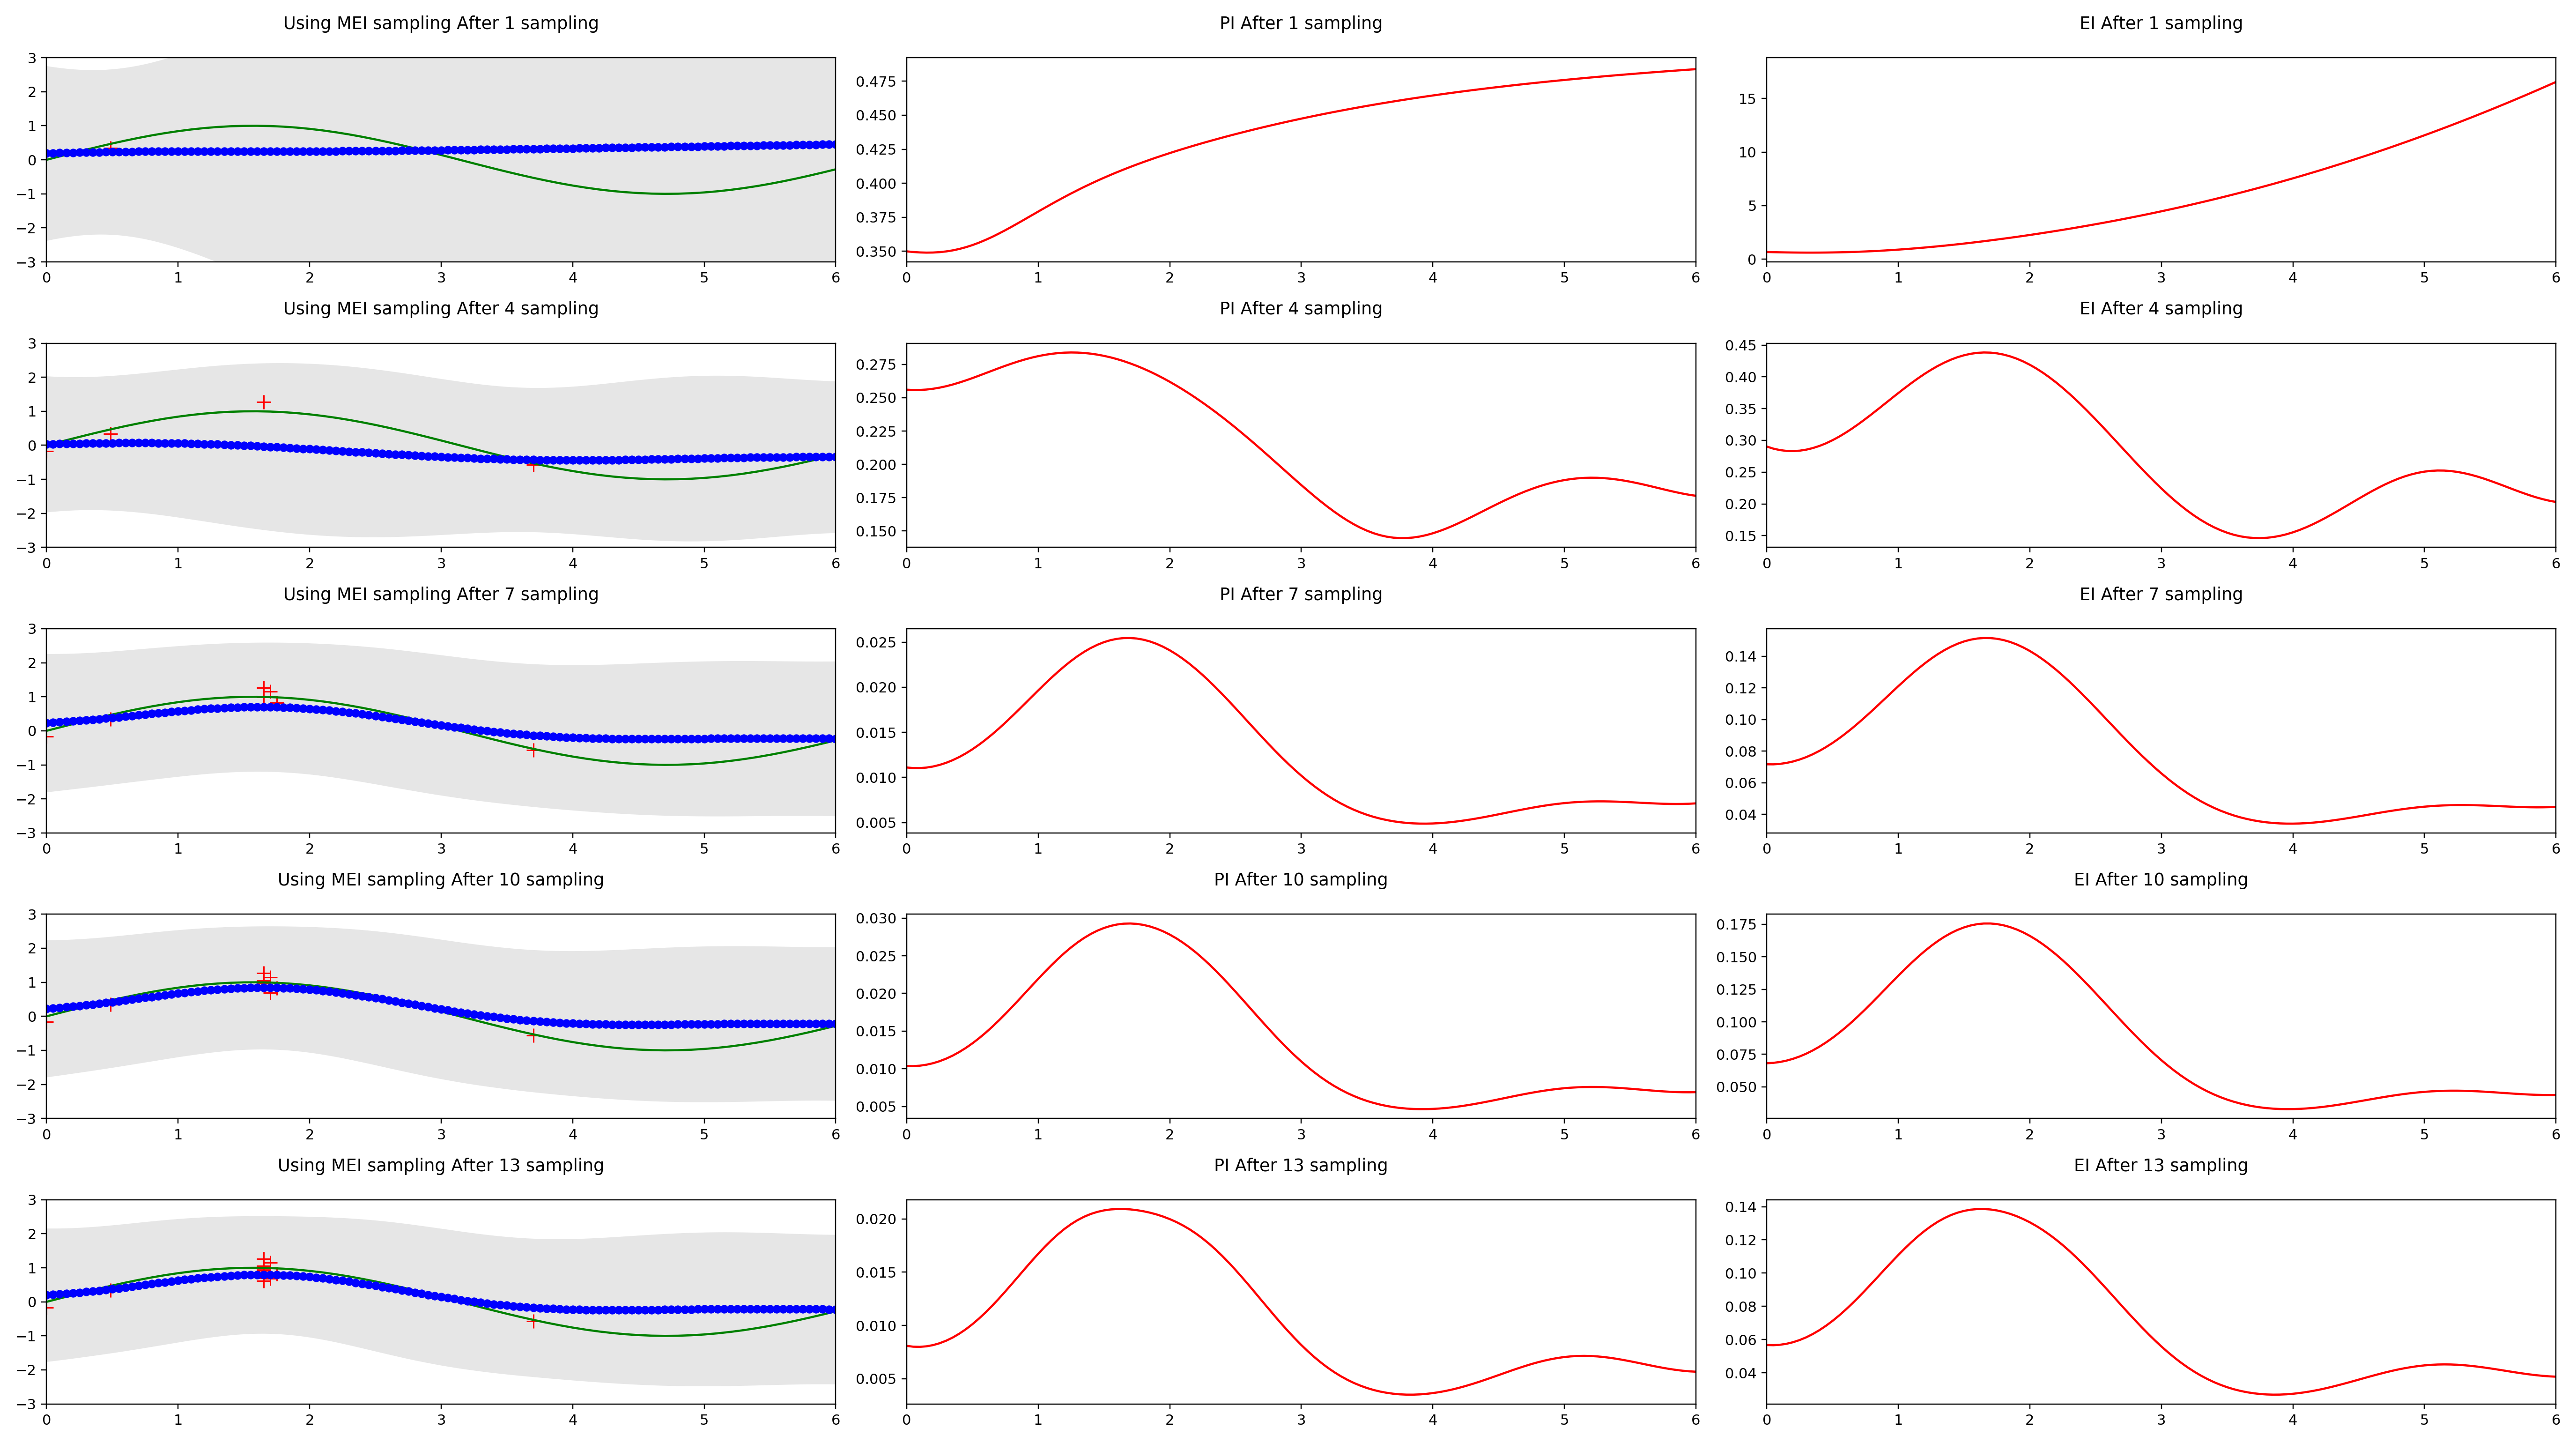
\includegraphics[scale=0.2]{fig12_28.png} 
\caption{MEI 샘플링 과정}
\label{fig:12-21}
\end{figure}

\end{document}